\documentclass[aspectratio=169,
				xcolor=table]{beamer}

% Load general definitions
\usepackage[utf8]{inputenc}
%\usepackage[T1]{fontenc}
\usepackage[brazil]{babel}
\usepackage{amsmath}
\usepackage{amsfonts}
\usepackage{amssymb}
\usepackage{graphicx}
\usepackage{verbatim}
\usepackage{cancel}
\usepackage{askmaps}
\usepackage{tabularx}
\usepackage[table]{xcolor}
%\usepackage{tikz}
\usepackage{multirow}
\usepackage{mathtools}
\usepackage{color, colortbl}
\usepackage{etoolbox}
\usepackage{pbox}
\usepackage{changepage}
\usepackage{xpatch}
\usepackage{array}
\usepackage{marvosym}
\usepackage{tabu}
\usepackage{multicol}
\usepackage{listings}
\usepackage{underscore}
\usepackage{filecontents}
\usepackage[]{algorithm2e}
\usepackage{ragged2e}

\newcolumntype{P}[1]{>{\centering\arraybackslash}m{#1}}
\definecolor{Gray}{gray}{0.75}
\definecolor{Gray2}{gray}{0.85}

\definecolor{lightBlue}{HTML}{DAE8FC}
\definecolor{Blue}{RGB}{51, 51, 204}

%\useinnertheme[lily]{rounded}
\usetheme{UniEvangelica}
%\usetheme{Copenhagen}
%\usetheme{Berlin}
%\usecolortheme{dolphin}
\tolerance=1
\emergencystretch=\maxdimen
\hyphenpenalty=10000
\hbadness=10000

\setbeamertemplate{navigation symbols}{}%remove navigation symbols


\let\olditem=\item% 
\renewcommand{\item}{\olditem \justifying}%
\def\center{\trivlist \centering\item\relax}
\def\endcenter{\endtrivlist}

\setbeamertemplate{itemize/enumerate body begin}{\large}
\setbeamertemplate{itemize/enumerate subbody begin}{\large}

\setbeamertemplate{itemize item}{\raisebox{0.1ex}{$\blacktriangleright$}\hskip0.1em}
\setbeamertemplate{itemize subitem}{\raisebox{0.1ex}{$\blacktriangleright$}\hskip0.1em}

\newcommand{\greenarrow}{\textcolor{green}{\rotatebox[origin=c]{180}{\MVArrowDown}}}

\newcommand{\redarrow}{\textcolor{red}{\MVArrowDown}}

%\newcommand{\ftable}{
%	\begin{table}
%		\large
%		\centering
%		\rowcolors{1}{\ifnumless{\rownum}{2}{Blue}{lightBlue}}{}
%}

\newenvironment{eftable}{
	\begin{table}
		\large
		\centering
		\rowcolors{1}{}{Blue}
		\rowcolors{1}{\ifnumless{\rownum}{2}{Blue}{lightBlue}}{}
	}
	{
	\end{table}
}


%\setbeamertemplate{frametitle}
%{
%	%\vspace*{-2em}	
%	\insertframetitle
%
%	 %\textcolor{white}{\LARGE \insertframetitle}
%
%}

% Specific definitions

\institute[]{\uppercase{Engenharia de Software}}
\title[]{Arquitetura e Organização de Computadores}
\subtitle[]{\uppercase{História dos Computadores}}
\author[]{Prof. Alexandre Tannus}
\date{}

\AtBeginSection{\frame{\tableofcontents[currentsection]}}

\begin{document}
	\begin{frame}
		\titlepage
	\end{frame}

	\begin{frame}{Objetivos}
		\begin{itemize}
			\item Conhecer a evolução da computação, sob o ponto de vista do \textit{hardware}, \textit{software} e linguagens de programação 
			\vspace{1em}
			\item Compreender a Lei de Moore e seu impacto no desenvolvimento da computação
		\end{itemize}
	\end{frame}
	
%	\begin{frame}{Metodologia}
%		\begin{itemize}
%			\item O tema da aula é exposto pelo professor em sala de aula. Os alunos interagem durante a apresentação para resolução de dúvidas e exposição de questionamentos relevantes ao tema, os quais podem ser sanados diretamente pelo professor ou serem colocados em discussão pela turma. 
%			\vspace{1em}
%			\item Ao final da exposição do conteúdo são resolvidos exercícios de fixação, para melhor compreensão do tema. As questões podem ser retiradas de concursos públicos, ENADE, POSCOMP ou de autoria do próprio professor.
%		\end{itemize}
%	\end{frame}

	\begin{frame}
		\tableofcontents
	\end{frame}	
	
	\section{Máquinas Mecânicas}
	\begin{frame}
		\frametitle{Máquinas Mecânicas}
		\begin{itemize}
			\item Ábaco
			\item Ossos de Napier
			\item Pascaline
			\item Máquina de Babbage
			\item Máquina de Turing
		\end{itemize}
	\end{frame}
	
	\begin{frame}
		\frametitle{Ábaco}
		\begin{itemize}
			\item Instrumento de cálculo matemático 
			\item Desenvolvido na Mesopotâmia no século XXV a.C.
		\end{itemize}
		\begin{figure}
			\centering
			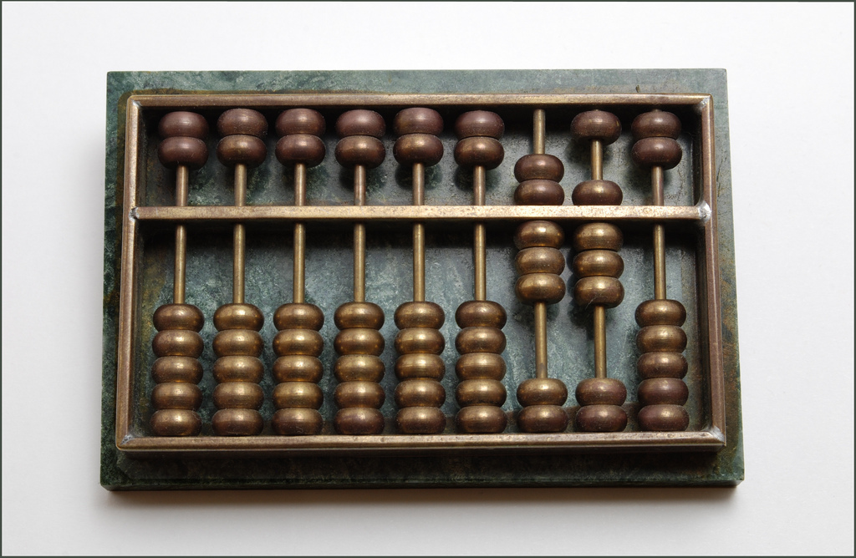
\includegraphics[width=0.4\textwidth, keepaspectratio]{../figs/cap03/abaco} 		
		\end{figure}
	\end{frame}

	\begin{frame}
		\frametitle{Ossos de Napier}
		\begin{itemize}
			\item Dispositivo para cálculo de multiplicação e divisão 
			\item Criado por John Napier 
		\end{itemize}
		\begin{figure}
			\centering
			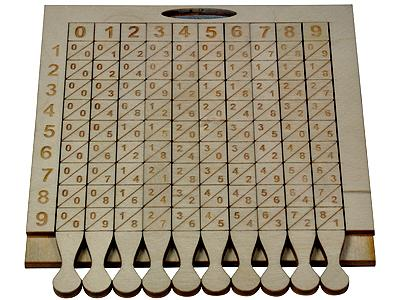
\includegraphics[width=0.4\textwidth, keepaspectratio]{../figs/cap03/napier} 		
		\end{figure}
	\end{frame}

	\begin{frame}
		\frametitle{Pascaline}
		\begin{itemize}
			\item Máquina de calcular mecânica 
			\item Desenvolvida por Blaise Pascal (1642) 
		\end{itemize}
		\begin{figure}
			\centering
			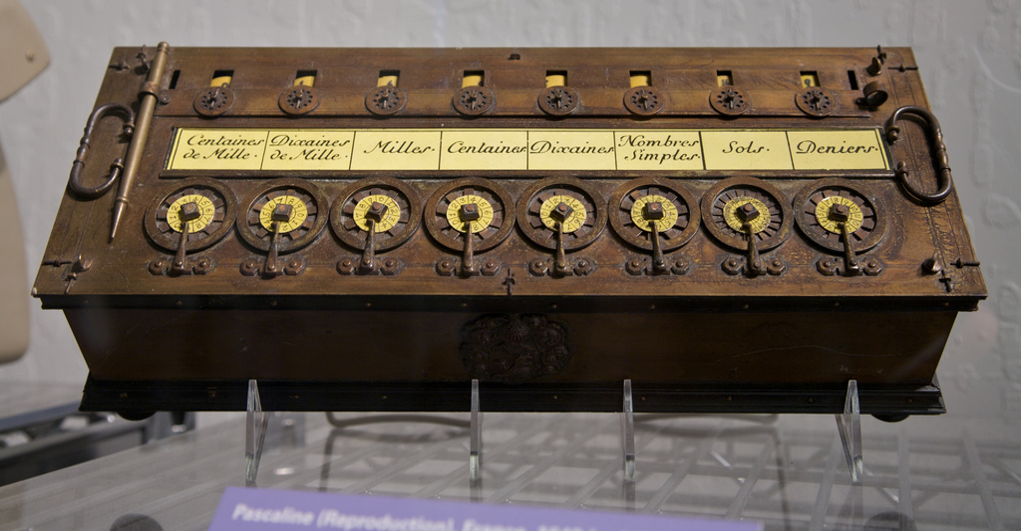
\includegraphics[width=0.6\textwidth, keepaspectratio]{../figs/cap03/pascaline} 		
		\end{figure}
	\end{frame}
	
	\begin{frame}
		\frametitle{Charles Babbage}
		\begin{columns}
			\begin{column}{0.6\textwidth}
				\begin{itemize}
					\item Matemático inglês (1791 – 1871)
					\vspace{1em}
					\item Máquina diferencial (1821)
					\begin{itemize}
						\item Cálculos polinomiais
						\item Entrada de dados, processamento, armazenamento e exibição de resultados
					\end{itemize}
				\end{itemize}
			\end{column}
			\begin{column}{0.4\textwidth}
				\begin{figure}
					\centering
					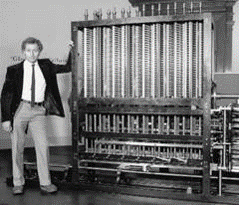
\includegraphics[width=0.9\textwidth, keepaspectratio]{../figs/cap03/babbage} 		
				\end{figure}
			\end{column}
		\end{columns}
	\end{frame}
	
	\begin{frame}
		\frametitle{Charles Babbage}
		\begin{columns}
			\begin{column}{0.6\textwidth}
				\begin{itemize}
					\item Engenho Analítico (1833 – 1871)
					\begin{itemize}
						\item Manipulador generalista de símbolos
						\item Precursor dos computadores modernos
						\item Nunca foi realmente montado
					\end{itemize}
				\end{itemize}
			\end{column}
			\begin{column}{0.4\textwidth}
				\begin{figure}
					\centering
					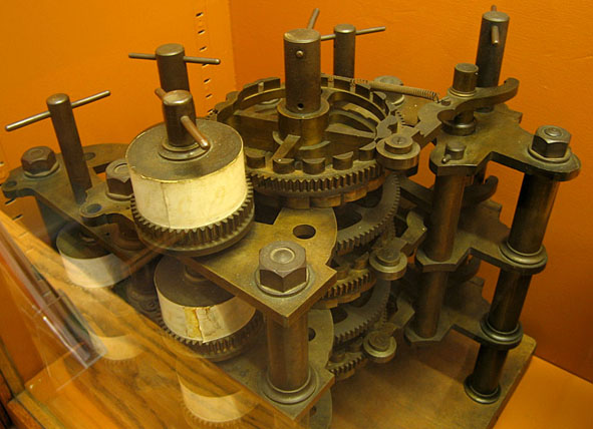
\includegraphics[width=0.9\textwidth, keepaspectratio]{../figs/cap03/babbage2} 		
				\end{figure}
			\end{column}
		\end{columns}
	\end{frame}	
	
	\begin{frame}
		\frametitle{Ada Lovelace}
		\begin{columns}
			\begin{column}{0.6\textwidth}
				\begin{itemize}
					\item Escritora e matemática inglesa

					\item Trabalhava com Charles Babbage

					\item Primeira pessoa a criar um algoritmo para uma máquina 
					\begin{itemize}
						\item Equação de Bernoulli
					\end{itemize}
				\end{itemize}
			\end{column}
			\begin{column}{0.4\textwidth}
				\begin{figure}
					\centering
					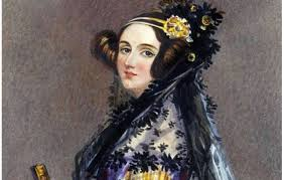
\includegraphics[width=0.9\textwidth, keepaspectratio]{../figs/cap03/ada} 		
				\end{figure}
			\end{column}
		\end{columns}
	\end{frame}	
	
	\begin{frame}
		\frametitle{Alan Turing}
		\begin{itemize}
			\item Matemático, criptoanalista e cientista da computação inglês (1912 – 1954)
			\vspace{1em}
			\item Contribuições importantes
			\begin{itemize}
				\item Enigma (decifrador de códigos de guerra alemães)
				\item Computador ACE 
				\item Criptografia de voz
				\item Teste de Turing
				\item Máquina de Turing
			\end{itemize}
		\end{itemize}
	\end{frame}
	
	\begin{frame}
		\frametitle{Máquina de Turing}
		\begin{itemize}
			\item Modelo teórico proposto em 1936
			\vspace{1em}
			\item Conceitos básicos de processamento, memória, armazenamento e entrada/saída de dados
			\begin{itemize}
				\item Dispositivo de leitura/escrita de dados em uma fita infinita
				\item Máquina de estados realiza operações na fita
			\end{itemize}
		\end{itemize}
	\end{frame}
	
	\begin{frame}
		\frametitle{Máquina de Turing}
		\begin{itemize}
			\item Operações disponíveis
			\begin{itemize}
				\item Leitura de símbolo
				\item Escrita de símbolo
				\item Movimentação da fita para a esquerda
				\item Movimentação da fita para a direita
				\item Mudar de estado
				\item Desligar
			\end{itemize}
		\end{itemize}
	\end{frame}
	
	\begin{frame}
		\frametitle{Teste de Turing – Capacidades da Máquina}
		\begin{itemize}
			\item Processamento de linguagem natural
			\begin{itemize}
				\item Entendimento do idioma falado pelo interlocutor
			\end{itemize}
			\vspace{1em}
			\item Representação do conhecimento
			\begin{itemize}
				\item Armazenamento das percepções do ambiente
			\end{itemize}
			\vspace{1em}
			\item Raciocínio automatizado
			\begin{itemize}
				\item Responder perguntas, realizar inferências e tirar conclusões
			\end{itemize}
		\end{itemize}
	\end{frame}	

	\begin{frame}
		\frametitle{Teste de Turing – Capacidades da Máquina}
		\begin{itemize}
			\item Aprendizado de máquina
			\begin{itemize}
				\item Adaptação a novas situações e detecção de novos padrões
			\end{itemize}
			\vspace{1em}
			\item Visão computacional
			\begin{itemize}
				\item Percepção de objetos no ambiente
			\end{itemize}
			\vspace{1em}
			\item Robótica
			\begin{itemize}
				\item Manipulação de objetos e movimentação
			\end{itemize}
		\end{itemize}
	\end{frame}	
	
	\section{1${}^a$ Geração}
	
	\begin{frame}[t]{Primeira Geração}
		\begin{columns}[t]
			\begin{column}{0.65\textwidth}
				\begin{itemize}
					\item 1946 – 1954 
					\vspace{1em}
					\item Válvulas e relés
					\vspace{1em}
					\item Programação em cartões perfurados
				\end{itemize}
			\end{column}
			\begin{column}{0.35\textwidth}
				\begin{figure}
					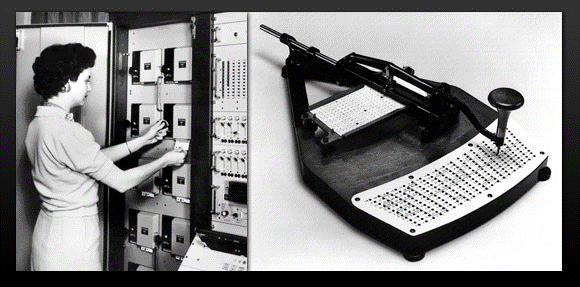
\includegraphics[width=0.9\textwidth, keepaspectratio]{../figs/cap03/geracao11} 			
				\end{figure}
				\begin{figure}
					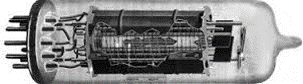
\includegraphics[width=0.9\textwidth, keepaspectratio]{../figs/cap03/geracao12} 			
				\end{figure}
			\end{column}
		\end{columns}
	\end{frame}

	\begin{frame}[t]{Primeira Geração}
		\begin{columns}[t]
			\begin{column}{0.6\textwidth}
				\begin{itemize}
					\item ENIAC - \textit{Electronic Numerical Integrator And Computer}
					\begin{itemize}
						\item John Mauchly e J. Presper Eckert
						\item $167 m^2$
						\item 30 toneladas
						\item 150 kW
						\item \textit{Clock}: 5000 Hz
						\item RAM: 83 bytes
					\end{itemize}
				\end{itemize}
			\end{column}
			\begin{column}{0.4\textwidth}
				\begin{figure}
					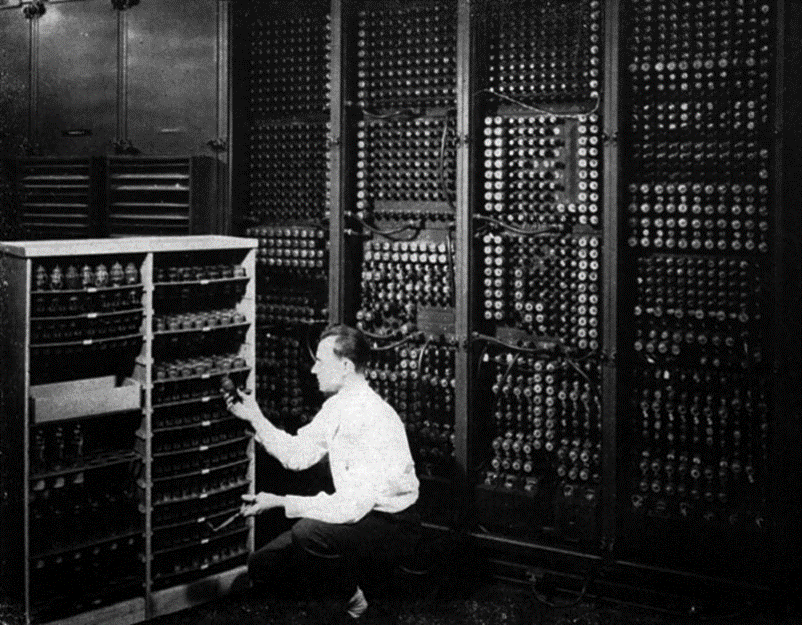
\includegraphics[width=0.9\textwidth, keepaspectratio]{../figs/cap03/eniac} 			
				\end{figure}
			\end{column}
		\end{columns}
	\end{frame}
	
	\section{2${}^a$ Geração}
	\begin{frame}[t]{Segunda Geração}
		\begin{itemize}
			\item 1955 - 1964 
			\vspace{1em}
			\item Utilização de Transistores 
			\vspace{1em}
			\item Armazenamento em disco e fita magnética
		\end{itemize}

		\vspace{-1em}
		\begin{columns}
			\begin{column}{0.65\textwidth}
				\begin{figure}
					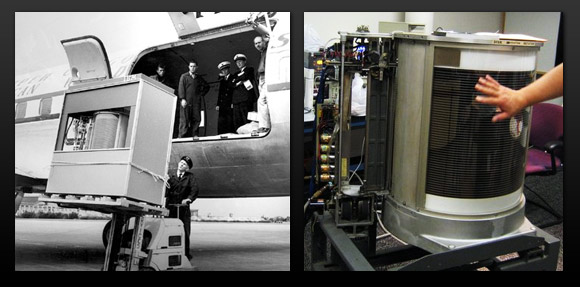
\includegraphics[height=3.5cm, keepaspectratio]{../figs/cap03/geracao22} 			
				\end{figure}
			\end{column}
			\begin{column}{0.35\textwidth}
				\begin{figure}
					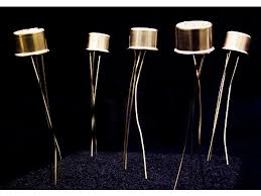
\includegraphics[width=0.9\textwidth, keepaspectratio]{../figs/cap03/geracao21} 			
				\end{figure}
			\end{column}
		\end{columns}
		
	\end{frame}

	\begin{frame}{Segunda Geração - Linguagens de Programação}
		\begin{itemize}
			\item Assembly
			\vspace{1em}
			\item Linguagens de alto nível
			\begin{itemize}
				\item \textbf{FOR}mula \textbf{TRAN}slation System (FORTRAN) – 1954 
				\item \textbf{LIS}t \textbf{P}rocessing (LISP) - 1958
				\item \textbf{CO}mmon \textbf{B}usiness \textbf{O}riented \textbf{L}anguage (COBOL) – 1959 
				\item \textbf{ALGO}rithmic \textbf{L}anguage  (ALGOL) – 1961 
				\item \textbf{B}eginner's \textbf{A}ll-purpose \textbf{S}ymbolic \textbf{I}nstruction \textbf{C}ode (BASIC) – 1963 
			\end{itemize}
		\end{itemize}
	\end{frame}
	
	\section{3${}^a$ Geração}
	\begin{frame}{Terceira Geração}
		\begin{columns}
			\begin{column}{0.65\textwidth}
			\begin{itemize}
				\item 1965 – 1977
				\vspace{1em}
				\item Circuitos integrados
				\begin{itemize}
					\item Milhares de transistores
					\item Aumento da capacidade de processamento
				\end{itemize}
			\end{itemize}
			\end{column}
			\begin{column}{0.35\textwidth}
				\begin{figure}
					\centering
					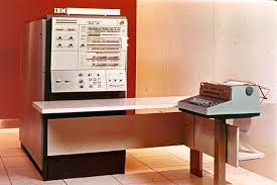
\includegraphics[height=3cm, keepaspectratio]{../figs/cap03/geracao31} 			
				\end{figure}
			\end{column}
		\end{columns}
		\vspace{-0.5em}
		\begin{figure}
			\centering
			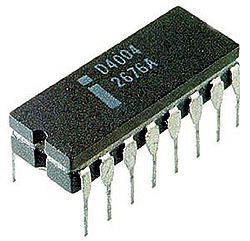
\includegraphics[height=3cm, keepaspectratio]{../figs/cap03/geracao32} 			
		\end{figure}
	\end{frame}	
	
	\begin{frame}{Terceira Geração}
		\begin{itemize}
			\item Popularização de FORTRAN e COBOL
			\vspace{1em}
			\item Desenvolvimento de novas linguagens
			\begin{itemize}
				\item PASCAL – 1970 – Niklaus Wirth 
				\item C – 1973 – Dennis Ritchie
			\end{itemize}
			\vspace{1em}
			\item Início dos estudos em redes de computadores
			\begin{itemize}
				\item ARPANET - 1969
				\item Ethernet – 1973 – Robert Metcalfe
				\item TCP/IP – 1976 – Vinton Cerf e Robert Kahn
			\end{itemize}

		\end{itemize}
	\end{frame}	
	
	\section{4${}^a$ Geração}
	\begin{frame}[t]{Quarta Geração}
		\begin{columns}[t]
			\begin{column}{0.7\textwidth}
			\begin{itemize}
				\item 1977 – 1991
				\vspace{1em}
				\item Desenvolvimento dos microprocessadores
				\begin{itemize}
					\item Integração em larga escala (VLSI)
				\end{itemize}
				\vspace{1em}
				\item Desenvolvimento dos microcomputadores
			\end{itemize}
			\end{column}
			\begin{column}{0.3\textwidth}
				\begin{figure}
					\centering
					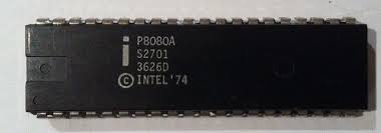
\includegraphics[width=0.9\textwidth, keepaspectratio]{../figs/cap03/geracao41} 			
				\end{figure}
				\begin{figure}
					\centering
					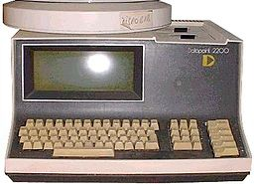
\includegraphics[height=3cm, keepaspectratio]{../figs/cap03/geracao42} 			
				\end{figure}				
			\end{column}
		\end{columns}
	\end{frame}

	\begin{frame}[t]{Quarta Geração}
		\begin{columns}[t]
			\begin{column}{0.65\textwidth}
				\begin{itemize}
					\item Sistemas operacionais
					\begin{itemize}
						\item Unix – 1977
						\item MS-DOS – 1981
						\item MacOS – 1984
					\end{itemize}
					\vspace{0.5em}
					\item Popularização do mouse
					\begin{itemize}
						\item Desenvolvido por Doug Engelbart (1961)
						\item Mouse de dois botões com bola – Jean-Daniel Nicoud(1974)
						\item Logitech (1981)
						\item Apple e Microsoft (1983)
					\end{itemize}
				\end{itemize}
			\end{column}
			\begin{column}{0.35\textwidth}
				\vspace{-1.5em}
				\begin{figure}
					\centering
					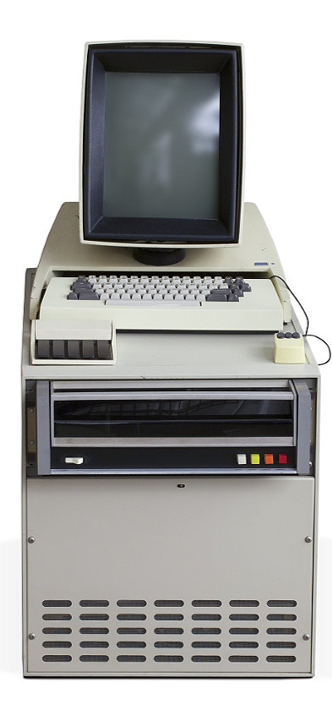
\includegraphics[height=6cm, keepaspectratio]{../figs/cap03/geracao43} 			
				\end{figure}			
			\end{column}
		\end{columns}
	\end{frame}

	\begin{frame}[t]{Quarta Geração}
		\begin{columns}[t]
			\begin{column}{0.5\textwidth}
				\begin{itemize}
					\item Interfaces gráficas de usuário (GUI)
					\begin{itemize}
						\item Xerox Alto – 1973 
						\item Xerox Star – 1981  
						\item Mac OS System 1 – 1984
						\item Windows 1.0 – 1985 
					\end{itemize}
				\end{itemize}
			\end{column}
			\begin{column}{0.5\textwidth}
				\begin{figure}
					\centering
					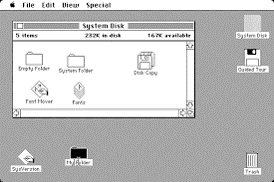
\includegraphics[width=\textwidth, keepaspectratio]{../figs/cap03/geracao44} 			
				\end{figure}
			\end{column}
		\end{columns}
	\end{frame}

	\begin{frame}
		\frametitle{Quarta Geração - Linguagens de Programação}
		\begin{columns}
			\begin{column}{0.5\textwidth}
				\begin{figure}
					\centering
					
\includegraphics[width=\textwidth, keepaspectratio]{../figs/cap03/linguagemcpp} 			
				\end{figure}
			\end{column}
			\begin{column}{0.5\textwidth}
				\vspace{-1em}
				\begin{figure}
					\centering
					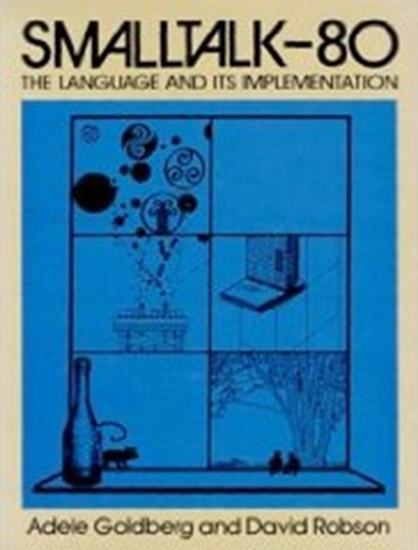
\includegraphics[height=6cm, keepaspectratio]{../figs/cap03/linguagemsmalltalk} 			
				\end{figure}
			\end{column}
		\end{columns}
	\end{frame}
	
	\begin{frame}[t]{Quinta Geração}
		\begin{columns}
			\begin{column}{0.65\textwidth}
				\begin{itemize}
					\item 1991 – Atualmente 
					\vspace{1em}
					\item Microprocessadores de 16, 32 e 64 bits
					\vspace{1em}
					\item Aumento de capacidade
					\begin{itemize}
						\item Unidades de armazenamento
						\item Memórias
						\item Procesamento
					\end{itemize}
				\end{itemize}
			\end{column}
			\begin{column}{0.35\textwidth}
				\vspace{-1em}
				\begin{figure}
					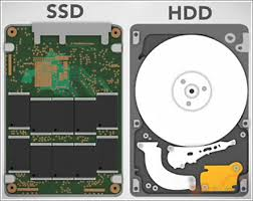
\includegraphics[width=0.8\textwidth, keepaspectratio]{../figs/cap03/geracao52} 			
				\end{figure}
				\vspace{-2em}
				\begin{figure}
					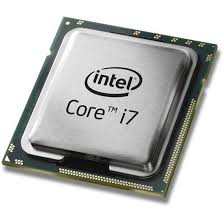
\includegraphics[width=0.6\textwidth, keepaspectratio]{../figs/cap03/geracao51} 			
				\end{figure}
			\end{column}
		\end{columns}
	\end{frame}		

	\section{5${}^a$ Geração}
	\begin{frame}
		\frametitle{Quinta Geração}
		\begin{itemize}
			\item Alta conectividade
			\vspace{1em}
			\item Mobilidade
		\end{itemize}
		\begin{columns}
			\begin{column}{0.23\textwidth}
				\begin{figure}
					\centering
					
\includegraphics[width=0.9\textwidth, keepaspectratio]{../figs/cap03/wifi} 			
				\end{figure}
			\end{column}
			\begin{column}{0.23\textwidth}
				\begin{figure}
					\centering
					
\includegraphics[width=0.9\textwidth, keepaspectratio]{../figs/cap03/bluetooth} 			
				\end{figure}
			\end{column}
			\begin{column}{0.23\textwidth}
				\begin{figure}
					\centering
					
\includegraphics[width=0.9\textwidth, keepaspectratio]{../figs/cap03/ethernet} 			
				\end{figure}
			\end{column}
			\begin{column}{0.23\textwidth}
				\begin{figure}
					\centering
					
\includegraphics[width=0.9\textwidth, keepaspectratio]{../figs/cap03/quatrog} 			
				\end{figure}
			\end{column}
		\end{columns}
	\end{frame}	
	
	\begin{frame}{Quinta Geração}
		\begin{itemize}
			\item Abertura da internet
			\begin{itemize}
			 	\item World Wide Web (www) – Tim Berners Lee (1991)
			 	\item Navegador Mosaic – Marc Andreesen
			 \end{itemize} 
			\vspace{1em}
			\item Linguagens
		\end{itemize}
		\vspace{-1em}
		\begin{columns}
			\begin{column}{0.23\textwidth}
				\begin{figure}
					\centering
					
\includegraphics[width=0.8\textwidth, keepaspectratio]{../figs/cap03/linguagemhtml} 			
				\end{figure}
			\end{column}
			\begin{column}{0.23\textwidth}
				\begin{figure}
					\centering
					
\includegraphics[width=0.8\textwidth, keepaspectratio]{../figs/cap03/linguagemphp} 			
				\end{figure}
			\end{column}
			\begin{column}{0.23\textwidth}
				\begin{figure}
					\centering
					
\includegraphics[width=0.8\textwidth, keepaspectratio]{../figs/cap03/linguagemjava} 			
				\end{figure}
			\end{column}
			\begin{column}{0.23\textwidth}
				\begin{figure}
					\centering
					
\includegraphics[width=0.8\textwidth, keepaspectratio]{../figs/cap03/linguagemcs} 			
				\end{figure}
			\end{column}
		\end{columns}
	\end{frame}		
	
	\section{Lei de Moore}
		
	\begin{frame}
		\frametitle{Lei de Moore}
		\begin{columns}
			\begin{column}{0.7\textwidth}
				\begin{itemize}
					\item Elaborada em 1965 por Gordon Earl Moore
					\begin{itemize}
						\item Número de transistores em microchips dobraria sem aumento no custo de produção durante 10 anos
					\end{itemize}
					\vspace{1em}
					\item Reformulação em 1975
					\begin{itemize}
						\item Duplicação do número de transistores a cada dois anos
						\item Posteriormente foi estabelecido o prazo de 18 a 24 meses 
					\end{itemize}
				\end{itemize}
			\end{column}
			\begin{column}{0.3\textwidth}
					\centering
				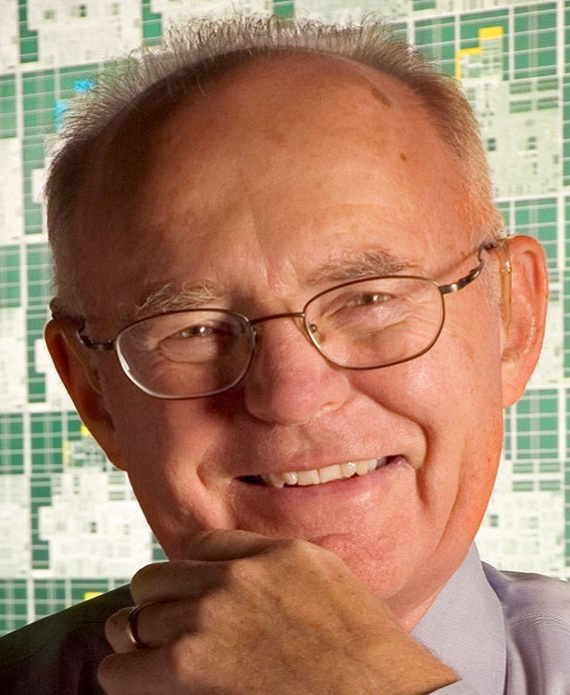
\includegraphics[height=5cm, keepaspectratio]{../figs/cap03/moore.png} 
			\end{column}
		\end{columns}
	\end{frame}
	
	\begin{frame}
		\frametitle{Lei de Moore}
		\begin{figure}
					\centering
			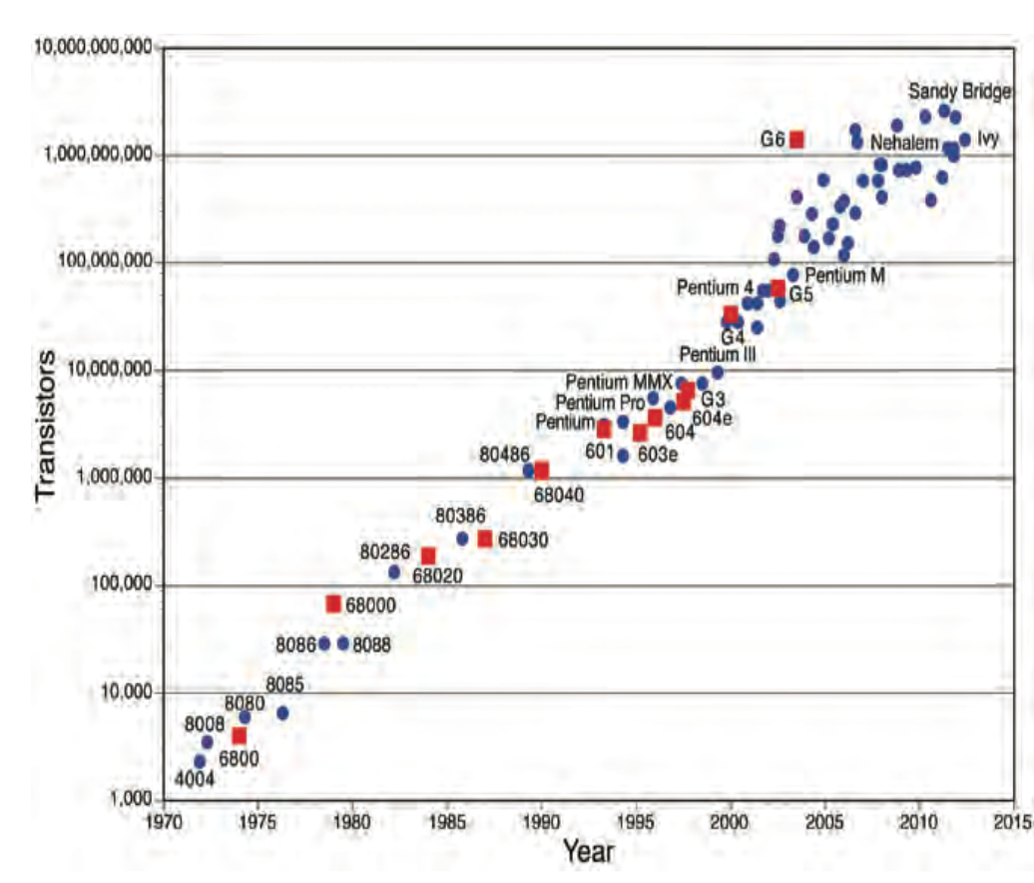
\includegraphics[height=6cm, keepaspectratio]{../figs/cap03/mooregrafico.png} 
		
		\end{figure}
	\end{frame}

	\begin{frame}
		\frametitle{\textit{Tick Tock}}
		\begin{figure}
					\centering
			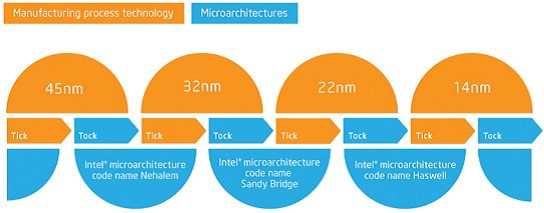
\includegraphics[width=0.9\textwidth, keepaspectratio]{../figs/cap03/ticktock.jpg} 
		\end{figure}
	\end{frame}
	
	\begin{frame}
		\frametitle{\textit{Process-Architecture-Optimization}}
		\begin{figure}
					\centering
			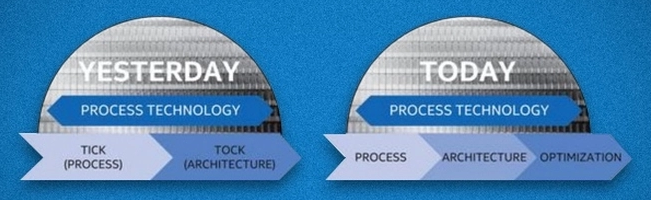
\includegraphics[width=\textwidth, keepaspectratio]{../figs/cap03/pao.png} 
		\end{figure}		
	\end{frame}
	
	\begin{frame}{Bibliografia}
		\nocite{Englander2011}
		\nocite{Paixao2014}
		\nocite{Stallings2010}
    	\bibliographystyle{plain}
    	\bibliography{../refs}   	
	
	\end{frame}
	
	\begin{frame}{}
		\end{frame}	
\end{document}